\documentclass[aps,prl,twocolumn,superscriptaddress,nofootinbib]{revtex4-1}

% the percent sign gives comments in Latex
% top line indicates this is for Physical Review, standard journal format,
% suitable for electronic submission of articles

% the line above is necessary to start any latex document.
% this is one variation that should work for most things.
% if you want double spaceing, use the following:
%
%\documentclass[prd,preprint,letterpaper]{revtex4}
%
% the "preprint" designation will make a wider line
% spacing, good for markup.
\usepackage{graphicx}  % this is the up-to-date package for all figures
\usepackage{amssymb}   % for math
\usepackage{verbatim}  % for the comment environment
\usepackage{color}
\usepackage{gensymb}
\usepackage{amsmath}

\usepackage[section]{placeins}

\usepackage{wrapfig}
\usepackage{hyperref}
\usepackage{titlesec}
\usepackage{amssymb}   % for math
\usepackage{verbatim}  % for the comment environment
\usepackage{color}
\usepackage[nodisplayskipstretch]{setspace}
\usepackage{amsmath}
\usepackage{blindtext}
%\usepackage[pdftex]{graphicx}
\usepackage[outdir=./]{epstopdf}
\usepackage[space]{grffile}
\usepackage{epsfig}
\usepackage[separate-uncertainty=true]{siunitx}
\usepackage{tikz}
\usepackage{pgfgantt}
\usepackage[english]{babel}
\usepackage[utf8]{inputenc}

\titlespacing*{\section}
{0pt}{1\baselineskip}{.5\baselineskip}

\titlespacing*{\subsection}
{0pt}{1\baselineskip}{.3\baselineskip}

\setlength{\textfloatsep}{1\baselineskip plus 0.2\baselineskip minus 0.5\baselineskip}

\usepackage{footnote}

\bibliographystyle{apsrev}


% these are some custom control of the page size and margins
% \topmargin= 0.2in  % these 1st two may be needed for some computers
% \textheight=8.75in
%\textwidth=6.5in
%\oddsidemargin=0cm
%\evensidemargin=0cm

% this is where the actual document itself (rather than control statements) begins:

\begin{document}

% use a style that gives automatic headings
%\pagestyle{headings}



% the \title{} command generates a title.

% the \\ below is used to FORCE a line break in the middle of the sentence--
% otherwise latex computes it for you

\title{Nuclear Magnetic Resonance}


\author{\textbf{Bryan Yamashiro}}
\author{Brandon Agtarap}
\author{Corey Mutnik}
\author{Daichi Hiramatsu}
%\author{Christina Nelson}

\affiliation{Department of Physics \& Astronomy, \\
University of Hawaii at Manoa,\\
2505 Correa Rd, Honolulu, HI, 96822, USA}





	      % \section is used to start a new one with a heading
\begin{abstract}

The relaxation times of heavy mineral oil are experimentally determined in this study. The nuclei of heavy mineral oil investigated are very abundant and give particularly strong signals.
The spin-lattice relaxation time is (24.5$\pm$0.9)\,ms and the spin-spin relaxation time is (18.2$\pm$1.5)\,ms.

%The sigma deviations of LiF ranged between 0.77$\sigma$ to 1.94$\sigma$. The low sigma results showed that the lithium fluoride quite accurately determined the lattice constant. Conversely, the sodium chloride sigma errors ranged between 2.27$\sigma$ to 3.28$\sigma$, which showed more deviation, but was still acceptable.



\end{abstract}

\maketitle    % this line is necessary to tell latex you are done with all
	      % of the stuff associated with the title, and now it can go
              % ahead and generate the title portion


\section{Background and Theory}
Nuclear Magnetic Resonance\,(NMR) spectroscopy was first utilized in 1946. The NMR technique is useful for studying physical phenomena from kinetics to superconductivity, and was recognized with a Nobel Prize in Physics\,\cite{1}. The major importance of NMR is the ability to characterize materials by probing the nuclei and immediate surroundings. Within a certain solid there are varieties of local magnetic fields, and NMR spectroscopy is able to measure the local field at atomic nuclei. NMR also has implications in the medical field, with Magnetic Resonance Imaging\,(MRI). The imaging technique allows physicians to produce noninvasive three dimensional images of blood flow patterns in both the brain and heart, and eventually hopes to pinpoint malignant tissue without biopsies\,\cite{2}.
\\
\indent Magnetic Resonance\,(MR) is observed in constituents that have both a magnetic moment\,($\mu$) and angular momentum\,(J). It's imperative to note that many, but not all, of the stable nuclei exhibit these traits. 
%Simply, the observed nuclei both have spin one-half, therefore each magnetization step will displace nuclei by 90\degree. The displacements are illustrated in figure\,\ref{magnet} for the 90\degree and 180\degree pulses.

\begin{figure}[h!]
  \begin{center}
\centerline{\includegraphics[width=2.5in]{magnet.png}}
\caption{ \small{The red arrow illustrates the 90\degree pulse, and the blue represents the 180\degree pulse. \label{magnet}}}
\end{center}
\end{figure}
\vfill\eject
The two magnetization states that are concerned in this study include the T$_1$ and the T$_2$ states. The initial magnetization is in the positive z-direction.
\begin{equation}
M_0=M_z
\end{equation}

T$_1$ is called the spin-lattice constant relaxation time, which requires a two pulse sequence. An initial 180\degree pulse flips the magnetization from M$_z$ to -M$_z$. The 180\degree pulse is followed by a 90\degree B pulse, which coverts the -M$_z$ state into the M$_{xy}$ plane-magnetization.
\\
\indent The T$_2$ state is called the spin-spin relaxation time. As the magnetization reaches the -M$_z$ state, the spin echo is triggered and an exponential decay is seen as time propagates. An initial 90\degree pulse turns M$_z$ to the M$_{xy}$ plane-magnetization. Following the initiation pulse, a secondary 180\degree pulse then changes the magnetization plane from M$_{xy}$ to -M$_{xy}$. Initial magnetization re-phases through the spin echo, and the time decay for this phenomena was measured as exponential decay.


 % the ~\cite{ } is how you link a reference in the text. The references
 % themselves are at the end.

% one or more lines of space between paragraphs determines them

\section{Apparatus}
The study used an apparatus, which a schematic is shown in figure\,\ref{scheme}, consisting mainly of a permanent magnet connected to a mainframe. The mainframe allowed for the manipulation of the A-pulse length\,(A\_len), B-pulse length\,(B\_len), tau\,($\tau$), iterations\,(Num\_B), period\,(P), and start pulse. A PS2 controller was connected to the mainframe to render various gradient configurations of the magnetic field. Voltage amplitudes were generated on the oscilloscope for data of relaxation calculations.

\begin{figure}[h]
    \begin{center}
    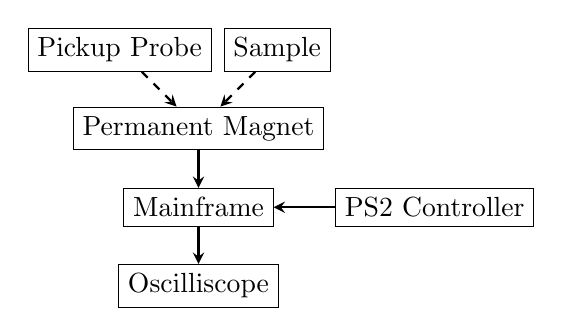
\begin{tikzpicture}[node distance=.3cm]
      %http://www.texample.net/tikz/examples/feature/arrows/
      \usetikzlibrary{shapes.geometric, arrows} 
      \tikzstyle{startstop} = [rectangle, rounded corners, minimum width=.2cm, minimum height=.2cm,text centered, draw=black]
      \tikzstyle{rect} = [rectangle, minimum width=.2cm, minimum height=.2cm, text centered, draw=black]%, fill=orange!30]
      \tikzstyle{parallelogram} = [diamond, minimum width=.2cm, minimum height=.2cm, text centered,draw=black]
      \tikzstyle{arrow} = [thick,->,>=stealth]
      \node (Aname) at (-2,5) [rect] {Sample};
      \node (Bname) at (-4,5) [rect] {Pickup Probe};
      \node (Cname) at (-3,4) [rect] {Permanent Magnet};
      \node (Dname) at (-3,3) [rect] {Mainframe};
      \node (Ename) at (0,3) [rect] {PS2 Controller};
      \node (Fname) at (-3,2) [rect] {Oscilliscope};


      \draw [dashed,arrow] (Aname) -- (Cname);
        \draw[dashed,arrow] (Bname) -- (Cname);
        \draw[arrow] (Cname) -- (Dname);
        \draw [arrow] (Ename) -- (Dname);
      \draw [arrow] (Dname) -- (Fname);

    \end{tikzpicture}
    \caption{\small{An illustration of the experimental setup. The dashed lines indicate the different samples that are input into the permanent magnet. \label{scheme}}}
    %\caption{\small{Schematic of experimental apparatus. \label{fig:aparatuslatex}}}
    \end{center}
  \end{figure}



\clearpage
\section{Procedure and Relevant Equations}

The sample used in this study was Heavy Mineral Oil\,(HIO). Initially, the NMR needed to be calibrated. Calibration was done using the Radio Frequency\,(RF) probe, and measuring the voltage outputs. HIO was prepared and placed into the magnetic field of the permanent magnet. A single pulse sequence consists of two bursts of RF magnetic field separated by a variable time, $\tau$. T1 was found by, an initial 180\degree pulse, followed by a 90\degree pulse. This two sequence procedure was iterated with varying times, $\tau$, between the A and B pulses. T2 was found by a pulse sequence of 90\degree to 180\degree\ to the echo maximum for a total time, 2$\tau$.



\begin{equation}
M_z =M_0(1-2e^{-\frac{t}{T_1}})
\label{t1eqn}
\end{equation}

The magnetization does not appear instantly, as there is a delay time between 90\degree and 180\degree pulses, so the observed quantities will portray an exponential growth, represented in equation\,\ref{t1eqn}. The instantaneous value, M, in equation\,\ref{t1eqn} represents the magnetization, while M$_0$ is the equilibrium value\,\cite{2}.

\begin{equation}
M_{xy}=M_0e^{\frac{-2t}{T_2}}
\label{t2eqn}
\end{equation}

Secondly, the T$_2$ state is the second degree magnetization. The exponential decay is represented in equation\,\ref{t2eqn}. The coefficient, 2, describes the progression from the 0\degree to 180\degree\,($\tau$) and from the 180\degree to spin echo\,(2$\tau$) state.




\section{Calculation of Results and Errors}
Figure\,\ref{T1unfig} was the original data that included the maximum amplitude of the Fee Induction Decay. To achieve the generated fit, the amplitudes before the minimum were flipped to negative amplitudes, resulting in figure\,\ref{T1fig}. The fits in equations\,\ref{t1eqn} and \ref{t2eqn} yielded computed results of the relaxation times. T$_1$ and T$_2$ were determined to be (24.5$\pm$0.9)\,ms and (18.2$\pm$1.5)\,ms, respectively.


\begin{figure}[h!]
  \begin{center}
\centerline{\includegraphics[width=3.5in]{t1unflip.pdf}}
\caption{ \small{Original T1 mineral oil data before the initial pulses were flipped to negative voltages. Spin-lattice constant relaxation time, T1 fit for heavy mineral oil. \label{T1unfig}}}
\end{center}
\end{figure}

\begin{figure}[h!]
  \begin{center}
\centerline{\includegraphics[width=3.5in]{t1best.pdf}}
\caption{ \small{Spin-lattice constant relaxation time, T1 fit for heavy mineral oil. \label{T1fig}}}

\centerline{\includegraphics[width=3.5in]{t2best.pdf}}
\caption{ \small{Spin-spin relaxation time, T2 fit for heavy mineral oil. \label{T2fig}}}
  \end{center}
\end{figure}



 \begin{table}[h!] 
\caption{Resultant decay time for both T1 and T2 relaxation times.}
    %table caption at the top is standard
\label{t1}   % labels are used to refer to this in the text
 \begin{center}   % center the table on the page
    \begin{tabular}{|c|c|c|} \hline   % tabular environment 
Relaxation & Pulse  & Decay Time \\
  Time State& Sequence (\degree)  &   (ms)  \\ \hline \hline \hline
T1 & 180$\rightarrow$90 & 24.5$\pm$0.9\\ \hline
T2 & 90$\rightarrow$180 & 18.2$\pm$1.5 \\ \hline
     \end{tabular}
  \end{center}
\end{table}


\section{Discussion and Conclusion}
The spin-lattice constant relaxation time was found to be (24.5$\pm$0.9)\,ms. Additionally, the spin-spin relaxation time was determined to be (18.2$\pm$1.5)\,ms. There were no literature values for these decay times, therefore sigma deviations were not reported. Error was mainly resultant from the oscilloscope while reading voltages. The maximum jump observed was 0.45\,V, therefore that uncertainty was carried for each value. An analysis was conducted on a fluorine sample, but due to low resolution in data, this sample was nullified.
\vfill\eject

%\section{Acknowledgments}


% the following \setlength is to force the bibliography to have no
% paragraph indentations.Can use vairous units--cm are used here.
\setlength{\parindent}{0cm}

\begin{thebibliography}{99}  % the trailing 99 controls some obscure format--just use

\bibitem{1} \url{http://pubs.acs.org/doi/abs/10.1021/ac00054a716?journalCode=ancham}    % {\em } for emphasis, \textbf{ } for boldface

\bibitem{2} \url{http://www.outreach.phy.cam.ac.uk/camphy/xraydiffraction/xraydiffractionindex.htm}

%\bibitem{3} "Multichannel Analyzer (MCA) Application Software." Nuclear Applications Software|ORTEC Scientific Equipment. ORTEC. Web. 5 Nov. 2015.

%\bibitem{3} \url{http://pdg.lbl.gov/2012/tables/rpp2012-sum-leptons.pdf}




\end{thebibliography}




\end{document}

